\documentclass[
    paper=a4,
    % twocolumn,
    fontsize=11pt,
    DIV=calc,
    fleqn, 
]{scrreport}


%___________________________________________________________________
% Custom Packages

%___________________________________________________________________
% Check LuaLaTeX Compiler

\usepackage{iftex}
\ifLuaTeX
    \relax
\else
    \PackageError{preamble}{This template is only compatible with LuaLaTeX. Please change your compiler.}{}
\fi


%___________________________________________________________________
% Fonts and Symbols

\usepackage{amssymb, amsmath, mathtools, amsfonts} % must be loaded before unicode-math
\usepackage{unicode-math}

\defaultfontfeatures{
    Scale=MatchLowercase,   % scale font to serif lowercase letter
    Ligatures=TeX,          % enable kerning for better spacing between letters
    Kerning=On              % replace sequences (fi) with a single glyph
}

\IfFontExistsTF{Libertinus Serif}{%
    \setmainfont{Libertinus Serif}
    \setmonofont[Scale=MatchLowercase]{Libertinus Mono}% or JetBrains Mono, Fira Code
    \setsansfont[Scale=MatchLowercase]{Libertinus Sans}        
    \setmathfont[    % load font in math mode, macro provided by unicode math
        Scale=MatchLowercase, % scale font to serif lowercase letter
        BoldFont=*  % use the same font for bold math
    ]{libertinusmath-regular.otf}   % must point to .otf file
}{
    \PackageWarning{preamble}{falling back to default fonts. Consider adding 'Libertinus Serif' to your system fonts (e.g. https://github.com/alerque/libertinus).}
    % fallback to default fonts
}


\usepackage[dvipsnames]{xcolor}   % must be loaded before luacolor
\usepackage{luacolor}   % color with Luatex attributes
\usepackage[soul]{lua-ul}      % more text markup options with soul

\usepackage[nopatch=footnote]{microtype}    
\UseMicrotypeSet[protrusion]{basicmath}


%___________________________________________________________________
% Language

\usepackage{polyglossia}
\setdefaultlanguage{german}
\setotherlanguage{english}


%___________________________________________________________________
% Citation and Bibliography

\usepackage[
  backend=biber,              
  style=ieee,                 
]{biblatex}  
\addbibresource{../sources.bib}

\usepackage[
    autostyle=true,
    german=quotes
]{csquotes}                             % quote environment
\MakeOuterQuote{"}                         % make " active for csquotes


%___________________________________________________________________
% Additional Packages

\usepackage{scrhack}   % common fixes for KOMA and other packages

\usepackage{booktabs}                               % better table vlines
\usepackage{tabularx}                               % tables with pagewidth
\usepackage{longtable}
\usepackage{array}
\usepackage{multirow}

\usepackage{caption}
\usepackage{subcaption}

\usepackage[
    detect-all,
    locale=DE,
    locale=DE,
    mode=match,
    % per-mode-fraction,
    range-units=repeat,
    range-phrase={{~bis~}}
]{siunitx}
\sisetup{
  output-decimal-marker = {,},
%   group-separator = {.},
  detect-weight = true,
  detect-family = true
}
\DeclareSIUnit{\euro}{€}


%___________________________________________________________________
% Image Dimensions

% 1. GLOBAL DEFAULTS & KEEP-ASPECT-RATIO
%    Images are configured globally with a default width and maximum height. 
%    Because 'keepaspectratio' is enabled, an image scales up until it 
%    hits the first of these thresholds. 
%    
%    By default, figures scale to: width = \imagewidthfactor\columnwidth.
%    Extremely tall images will be safely capped at \imagemaxheight.
%
% 2. THE \columnwidth ISSUE
%    Because default values are expanded immediately in the preamble, images placed 
%    inside columns, minipages, or boxes will NOT automatically adapt to the 
%    nested container's smaller \columnwidth. They will mistakenly inherit the 
%    original, global page \columnwidth.
%
% *RECOMMENDATIONS:*
% -> Always explicitly set the image width locally using:
%    [width=\imagewidthfactor\columnwidth]
%    This forces LaTeX to recalculate the width based on the current context.
%
% -> Do not specify a local height. The global \imagemaxheight and 
%    'keepaspectratio' settings remain active, so letting the height adjust 
%    automatically ensures correct proportions without overflow.

% Target width factor relative to the current \columnwidth
\newcommand{\imagewidthfactor}{0.5} 
\newcommand{\imagemaxwidthfactor}{1}

% upper bound for image heigths.
\newcommand{\imagemaxheight}{\textheight}

\usepackage[    % svgsetup is not known in latexml
    inkscapelatex=false,    % dont render text inside svg with latex
    keepaspectratio,
    height=\imagemaxheight,
    width=\imagewidthfactor\columnwidth,
]{svg}

\usepackage{graphicx}
% Images grow until width or height limit is reached.
\setkeys{Gin}{
    keepaspectratio,
    height=\imagemaxheight,
    width=\imagewidthfactor\columnwidth,
}

\graphicspath{{media/}}  

\usepackage{float}              % set default figure placements
\floatplacement{figure}{htbp}
\floatplacement{table}{htbp}

% \usepackage[section]{placeins}          % prevent floats from moving to other sections


%___________________________________________________________________
% Colors

\definecolor{colorblue}{HTML}{0480CC}				% color for weblinks
\definecolor{colordarkblue}{HTML}{4C1DCC}			% no use case at the moment
\definecolor{colorgreen}{HTML}{26CC1B}				% color for citations
\definecolor{colorred}{HTML}{CC1204}				% color for pdf links
\definecolor{coloryellow}{HTML}{F0B707}			    % color for warnings


%___________________________________________________________________
% Listings


\usepackage{minted}

\setminted{
    % linenos,
    breaklines,
    fontsize=\small,
    bgcolor=gray!9,
    tabsize=4,
    autogobble,
    style=friendly
}


%___________________________________________________________________
% Page Layout

\usepackage{flushend}                   % balance columns on last page in twocolumn mode

\KOMAoptions{
    toc     =   listof,                                     % add table of figures in 
    % headsepline=true,                               % switch header rule
    numbers =   noendperiod,
}

\flushbottom      

\usepackage{scrlayer-scrpage}


%___________________________________________________________________
% Hyperlinks

\usepackage[open]{bookmark}         % fixes bookmarks in pdf when using hyperref
\usepackage{xurl}                                 % better url line breaks, must be loaded before hyperref
\usepackage{hyperref}

\hypersetup{
    bookmarksnumbered=true,
    bookmarksopen=true,
    pdfpagemode=UseOutlines,
    breaklinks=true,
    colorlinks=true,
    % Keep link colors visually calm.
    linkcolor=colorblue,
    urlcolor=colorblue,
    anchorcolor=colorblue,
    menucolor=colorblue,
    runcolor=colorblue,
    citecolor=colorgreen,
    filecolor=magenta,      
}

\urlstyle{same} % default font for urls


%___________________________________________________________________
% Custom Commands

\newenvironment{fixedfigure}{
    \begin{center}
    \addvspace{0.5\intextsep}
}{
    \addvspace{0.5\intextsep}
    \end{center}
}

\newcommand{\imagesource}[1]{\par\footnotesize\textbf{Quelle:}~#1}   	%   Quellen für Bilder
\newcommand{\imagelegend}[1]{\par\footnotesize\textbf{Legende:}~#1}

\newcommand{\missing}{%
    \textcolor{coloryellow}{MISSING}%
    \PackageWarning{JHstyle}{You used the 'missing' macro at this line. Remove it before finalising document}%
}
\newcommand{\improve}{%
    \textcolor{coloryellow}{IMPROVE}%
    \PackageWarning{JHstyle}{You used the 'improve' macro at this line. Remove it before finalising document}%
}

\newcommand{\figW}{0.9\textwidth}   % single figure default width
\newcommand{\subfigW}{0.48\textwidth} % two-column subfigures
\newcommand{\figGap}{0.02\textwidth}

\newcommand{\bigfigw}{0.48\textwidth}


%___________________________________________________________________
% Titlepage

\titlehead{
    Hochschule Karlsruhe\\
    University of Applied Sciences
}

\subject{Projektarbeit}

\title{Entwurf und Umsetzung eines PCB-Frontends zum Senden und Empfangen von Breitbandsignalen bei 2,5GHz}

\author{Jan Hoegen%
    \thanks{\href{mailto:hoja1028@h-ka.de}{hoja1028@h-ka.de}, Matrikelnummer: 82358.}
}

\date{\today}

\publishers{
    \begin{tabular}{ll}
        Betreuer:   &   Tristan Itschner\\
                    &   Niklas Zeller
    \end{tabular}
}

\hypersetup{
    pdftitle={SDR Analog Frontend},
    pdfauthor={Jan Hoegen}
}

\ihead{Jan Hoegen}
\ohead{SDR Analog Frontend}


%___________________________________________________________________
% Front Matter

\begin{document}

\maketitle

\tableofcontents


%___________________________________________________________________
% Main Matter

% \begin{abstract}
    \subsubsection*{Abstract}
    Test Text TEST.
    % Verschiedene Signale werden auf einem Mikrocontroller erzeugt und über einen Digital-Analog-Wandler (DAC) ausgegeben. In diesem Bericht wird die Theorie und Implementierung mithilfe von Standardbibliotheken und Wertetabellen beschrieben. Dabei werden Sinus-, Impuls- und Rechtecksignale mit verschiedenen Abtastraten betrachtet. Die Signale werden mit einem Oszilloskop und einer FFT-Analyse untersucht, um die Qualität der Signale zu bewerten.

\end{abstract}
\chapter{Motivation und Aufgabenstellung}

Ziel dieser Projektarbeit ist es, ein analoges Frontend für ein Software-Defined-Radio zu entwicklen mit der Aufgabe, Eingangs- und Ausgangssignale auf 
\chapter{Systematisches Konzept}

Das Blockschaltbild in Abbildung \ref{fig:blockschaltbild} zeigt den prinzipiellen Aufbau. Die Signale des SDR werden mit einem 1.5 GHz signal gemischt um sie entweder hoch oder runter zu transferrieren.

Dabei gilt der Zusammenhang

\begin{align}
    f_{\text{LO}} = k f_{\text{RF}} \pm f_{\text{IF}}, \quad k \in \mathbb{Z}
\end{align}

\begin{figure}
    \centering
    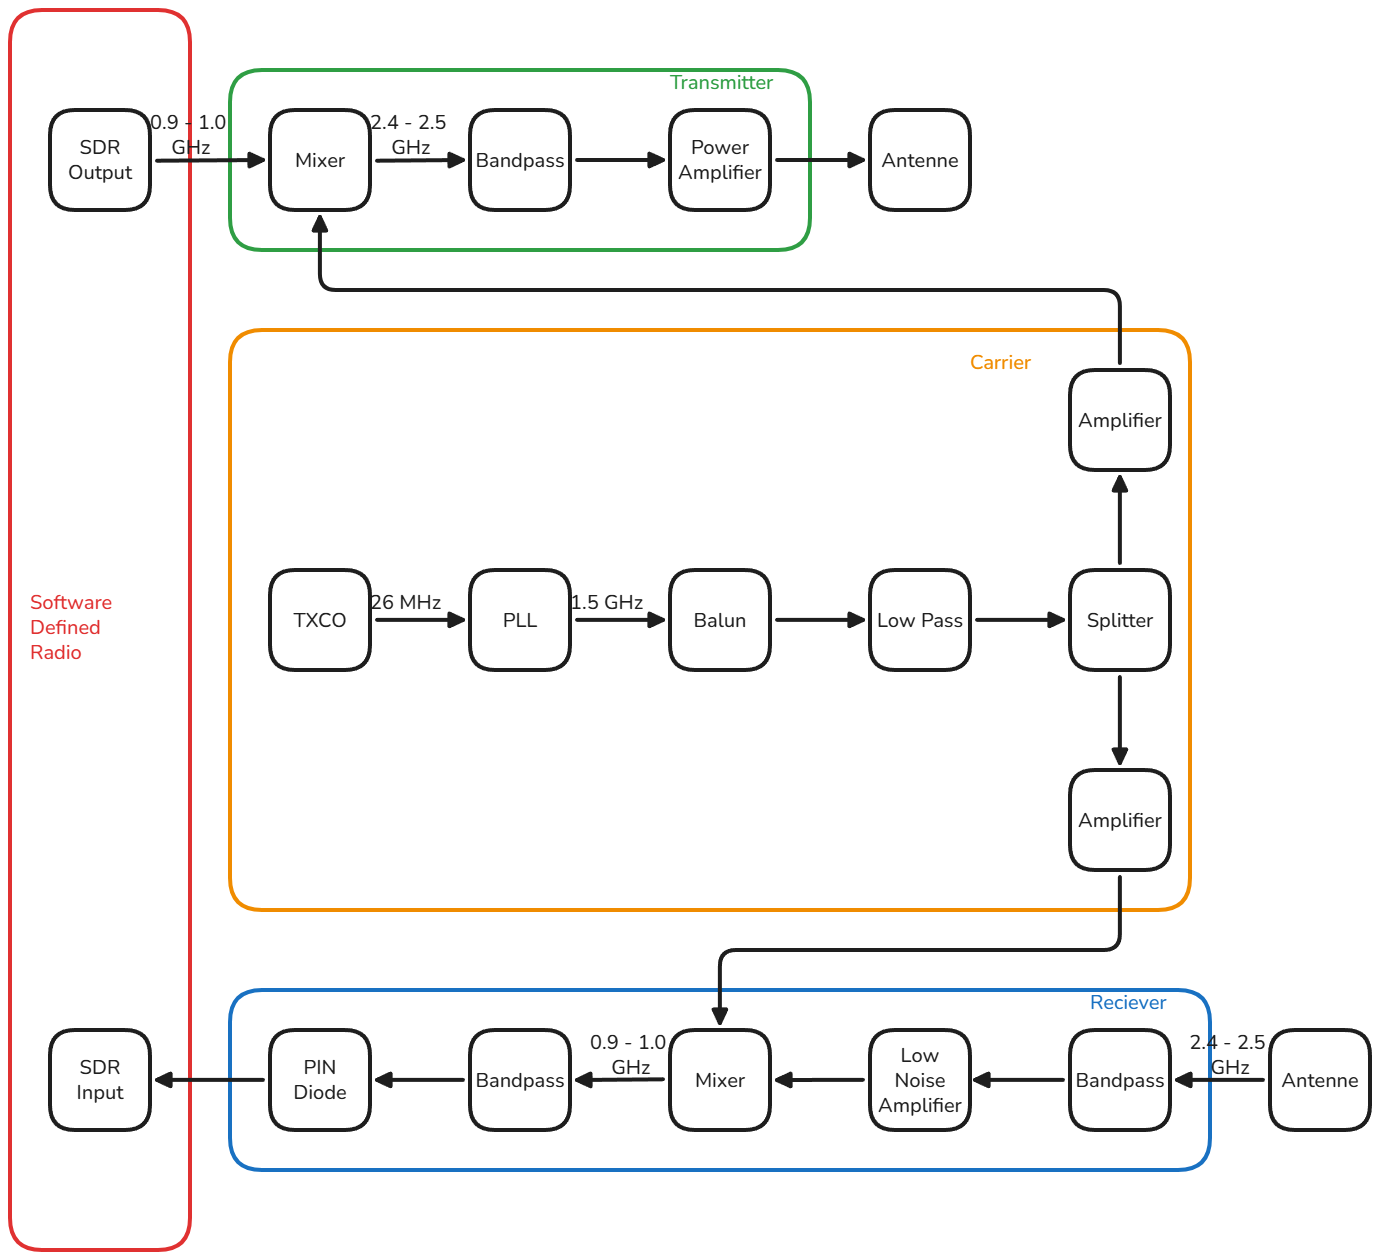
\includegraphics[width=\imagewidthfactor\columnwidth]{media/Blockschaltbild}
    \caption{Blockschaltbild des SDR Frontends.}
    \label{fig:blockschaltbild}
\end{figure}

\section{Oszillator Lösung}

Ein großes Problem war schwer zu lösen und hat daher den Zeitplan gesprengt: für 2.5 GHZ signale mit 900 MHz input ist eine Oszillatorfrequenz von 1.5 GHz notwendig. Kein VCO oder TXO kann diese mit Quatkristallen liefern. 

Mehrer Optionen wurden untersucht:


% TODO: tabelle mit oszillator optionen einfügen

Am ende wurde sich in Absprache mit dem Betreuer auf den PLL geeingigt. Damit stieg die komplexiztät für schematic, layout an. Am meisten wurde damit jedoch die Inbetriebnahme erschwert, da der ADF4351 erst mit einer SPI schnittstelle programmiert werden muss. 
\chapter{Simulation}

\begin{figure}
    \centering
    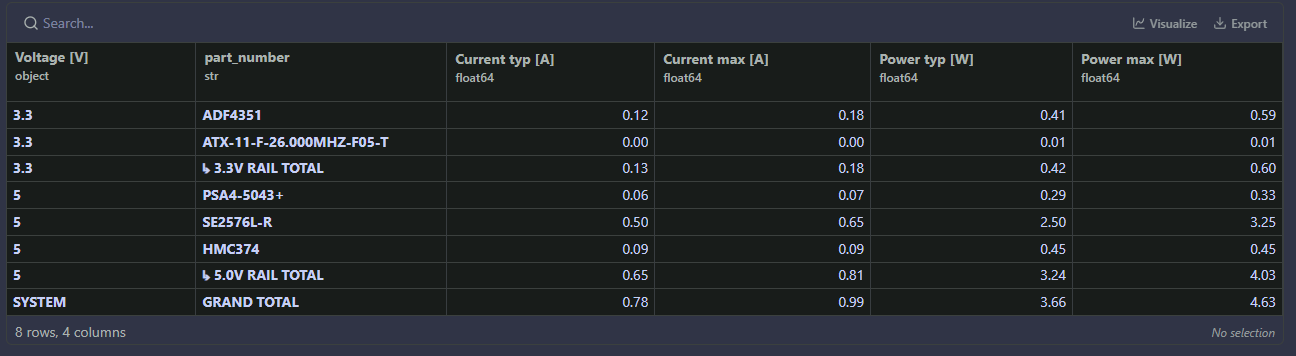
\includegraphics[width=\imagewidthfactor\columnwidth]{media/DC Power}
    \caption{Blockschaltbild des SDR Frontends.}
    % \label{fig:blockschaltbild}
\end{figure}

\begin{figure}
    \centering
    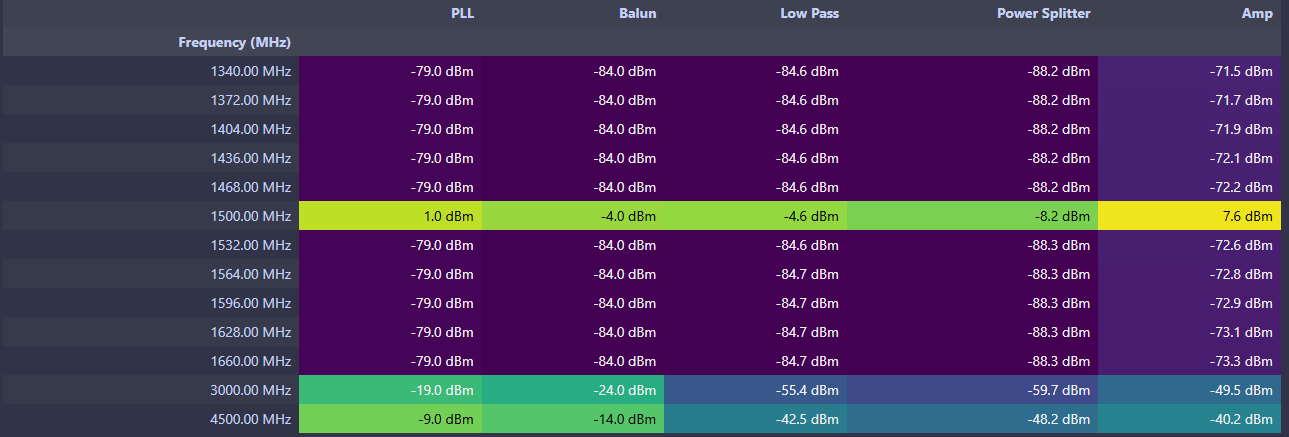
\includegraphics[width=\imagewidthfactor\columnwidth]{media/Oszillator}
    \caption{Blockschaltbild des SDR Frontends.}
    % \label{fig:blockschaltbild}
\end{figure}

\begin{figure}
    \centering
    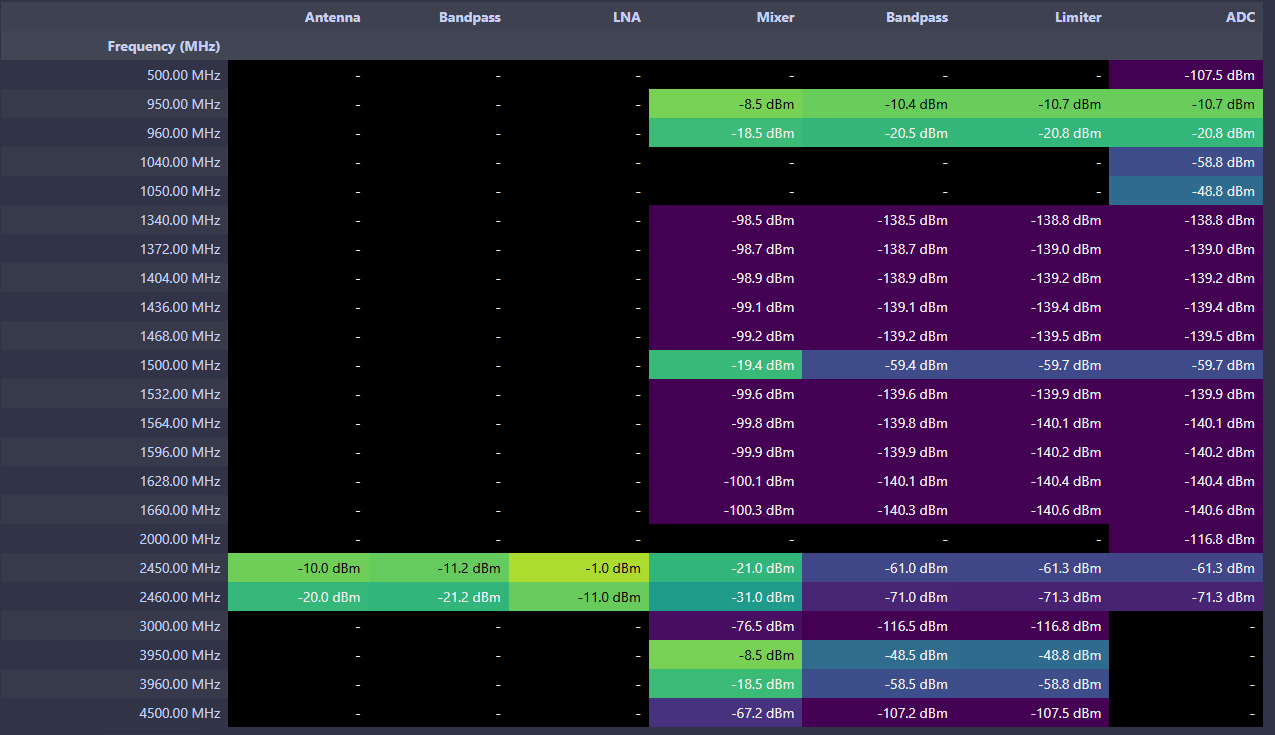
\includegraphics[width=\imagewidthfactor\columnwidth]{media/Receiver}
    \caption{Blockschaltbild des SDR Frontends.}
    % \label{fig:blockschaltbild}
\end{figure}

\begin{figure}
    \centering
    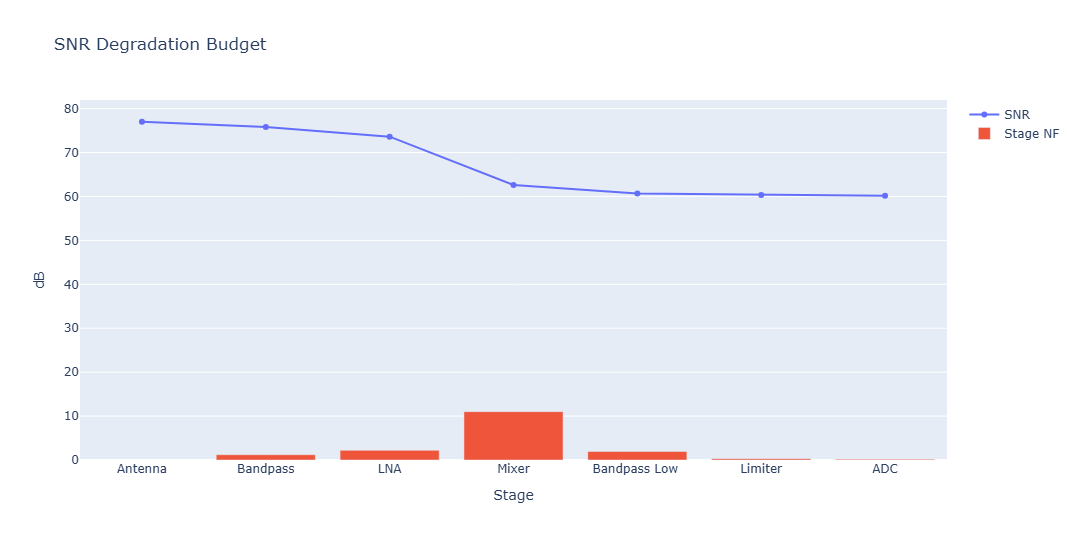
\includegraphics[width=\imagewidthfactor\columnwidth]{media/snr}
    \caption{Blockschaltbild des SDR Frontends.}
    % \label{fig:blockschaltbild}
\end{figure}

\begin{figure}
    \centering
    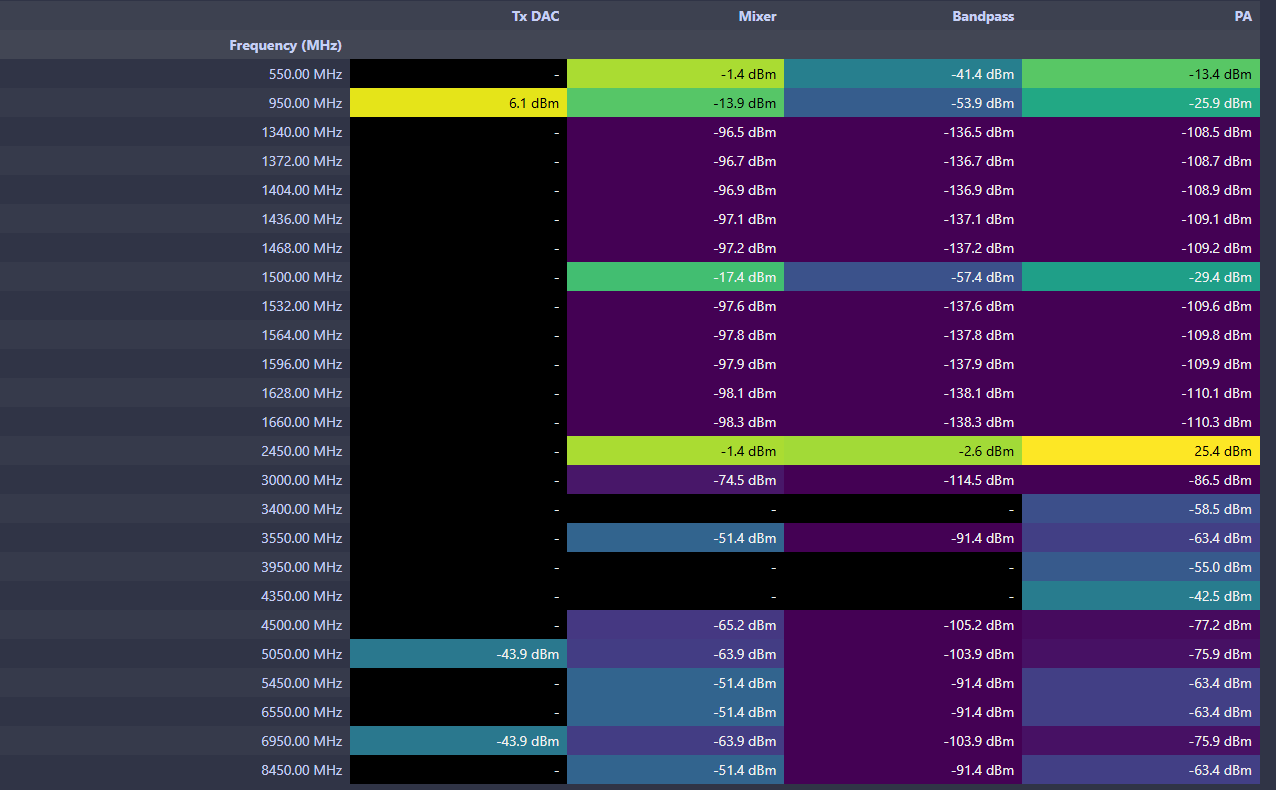
\includegraphics[width=\imagewidthfactor\columnwidth]{media/Transmitter}
    \caption{Blockschaltbild des SDR Frontends.}
    % \label{fig:blockschaltbild}
\end{figure}
\chapter{PCB Design und Layout}
\chapter{Vermessung}

vermessung ist gerade in progress.
\chapter{Fazit}

\section{Kosten}

% TODO: tabelle mit kosten einfügen

verstrichende Deadline erwähnen.

transmitter
    The RFSoC dac outputs a signal with max 40.5 mA current, output power -18.5 to 6.5 dBm.

    receiver
    the adc has maximum input power 14.6 dBm, input bandwidth 6 GHz and attenuation range 27 dB.


%___________________________________________________________________
% Back Matter

\appendix   % switches to heading letter numbering

\printbibliography[heading=bibnumbered]

\chapter{Verfügbarkeit des Codes}
    Die Code zur Simulation, die PCB Designdateien sowie die Dokumentation ist unter \href{https://git.ieem-ka.de/Jax/sdr-analog-frontend}{git.ieem-ka.de/Jax/sdr-analog-frontend} zu finden.
    Ebenso befindet sich der Quellcode zum Erstellen dieser Ausarbeitung und der Präsentation in diesem Repository.

    Für den Zugriff ist ein Account auf dem Gitlabinstanz notwendig.

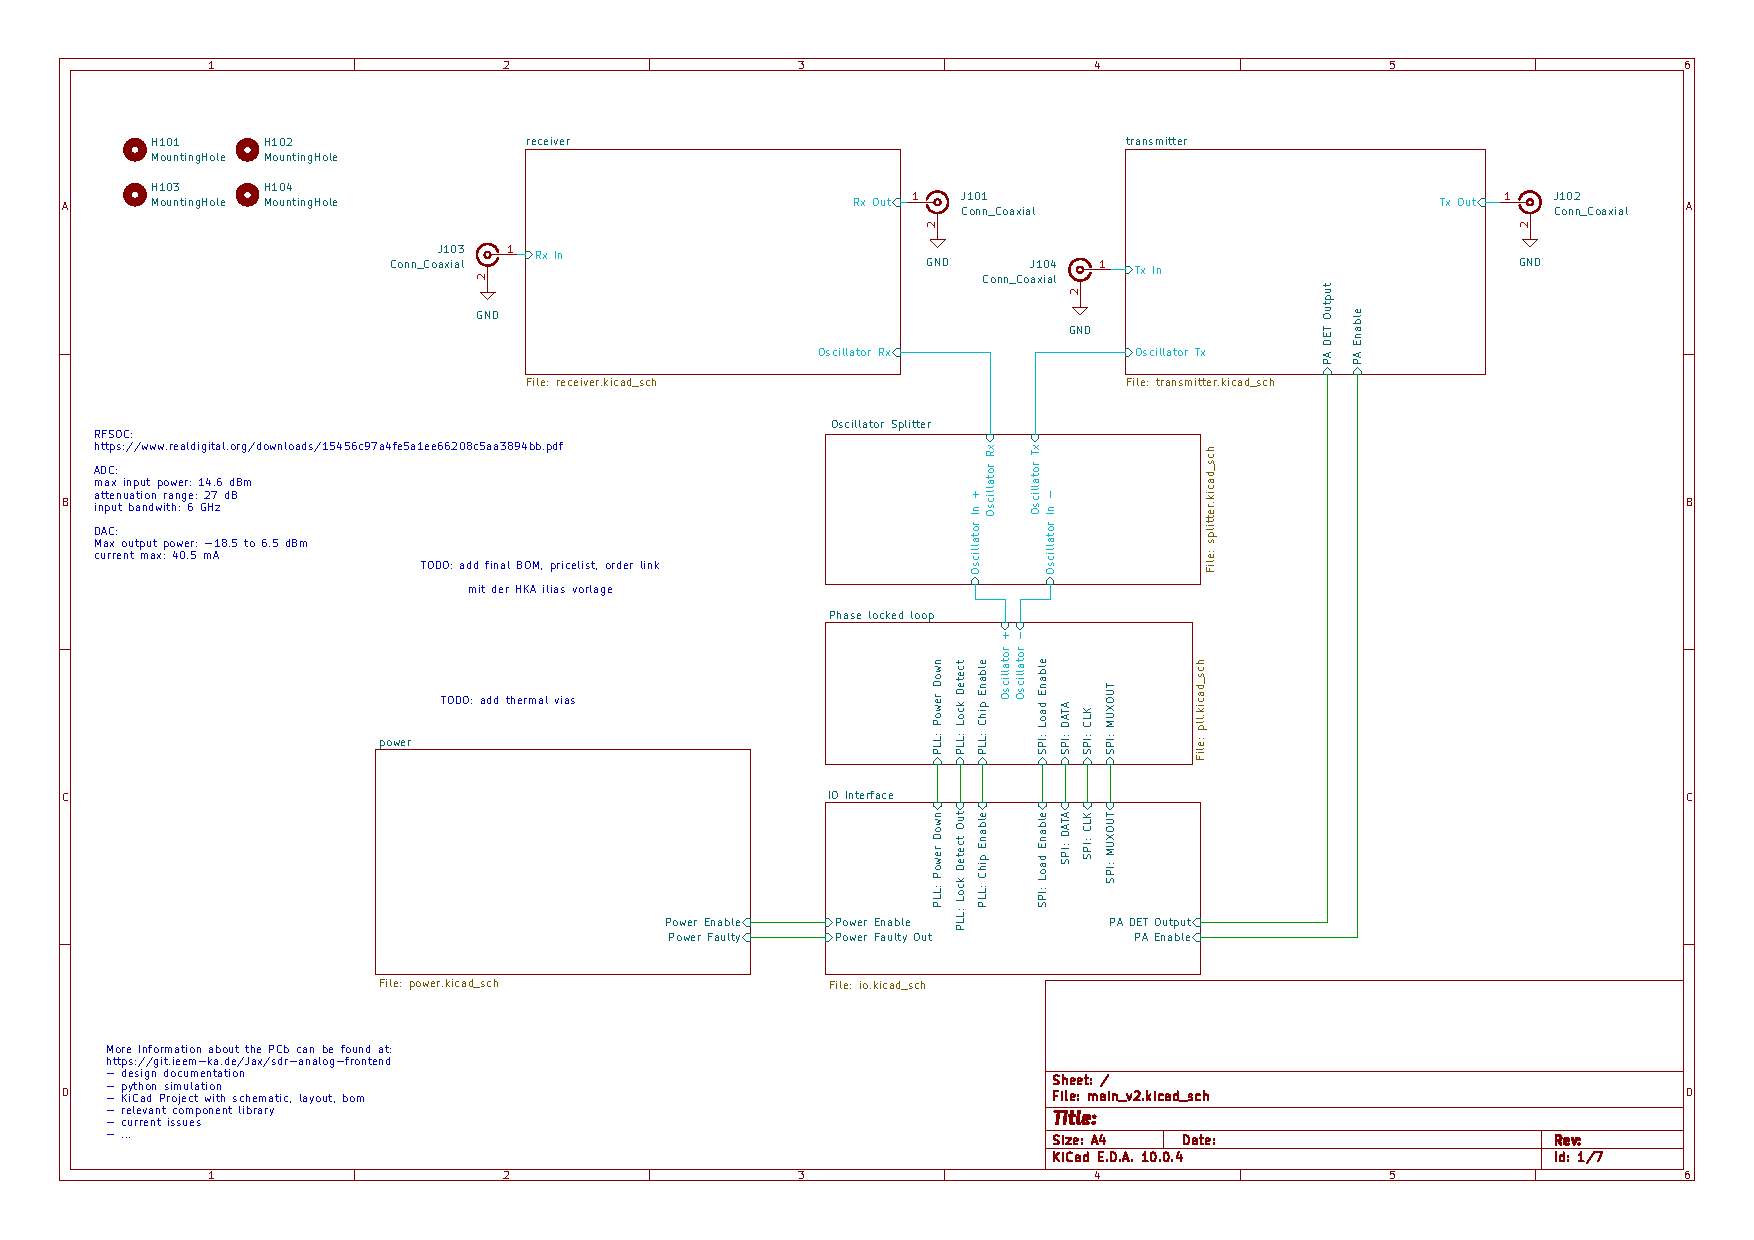
\includepdf[pages=-]{media/schematic.pdf}
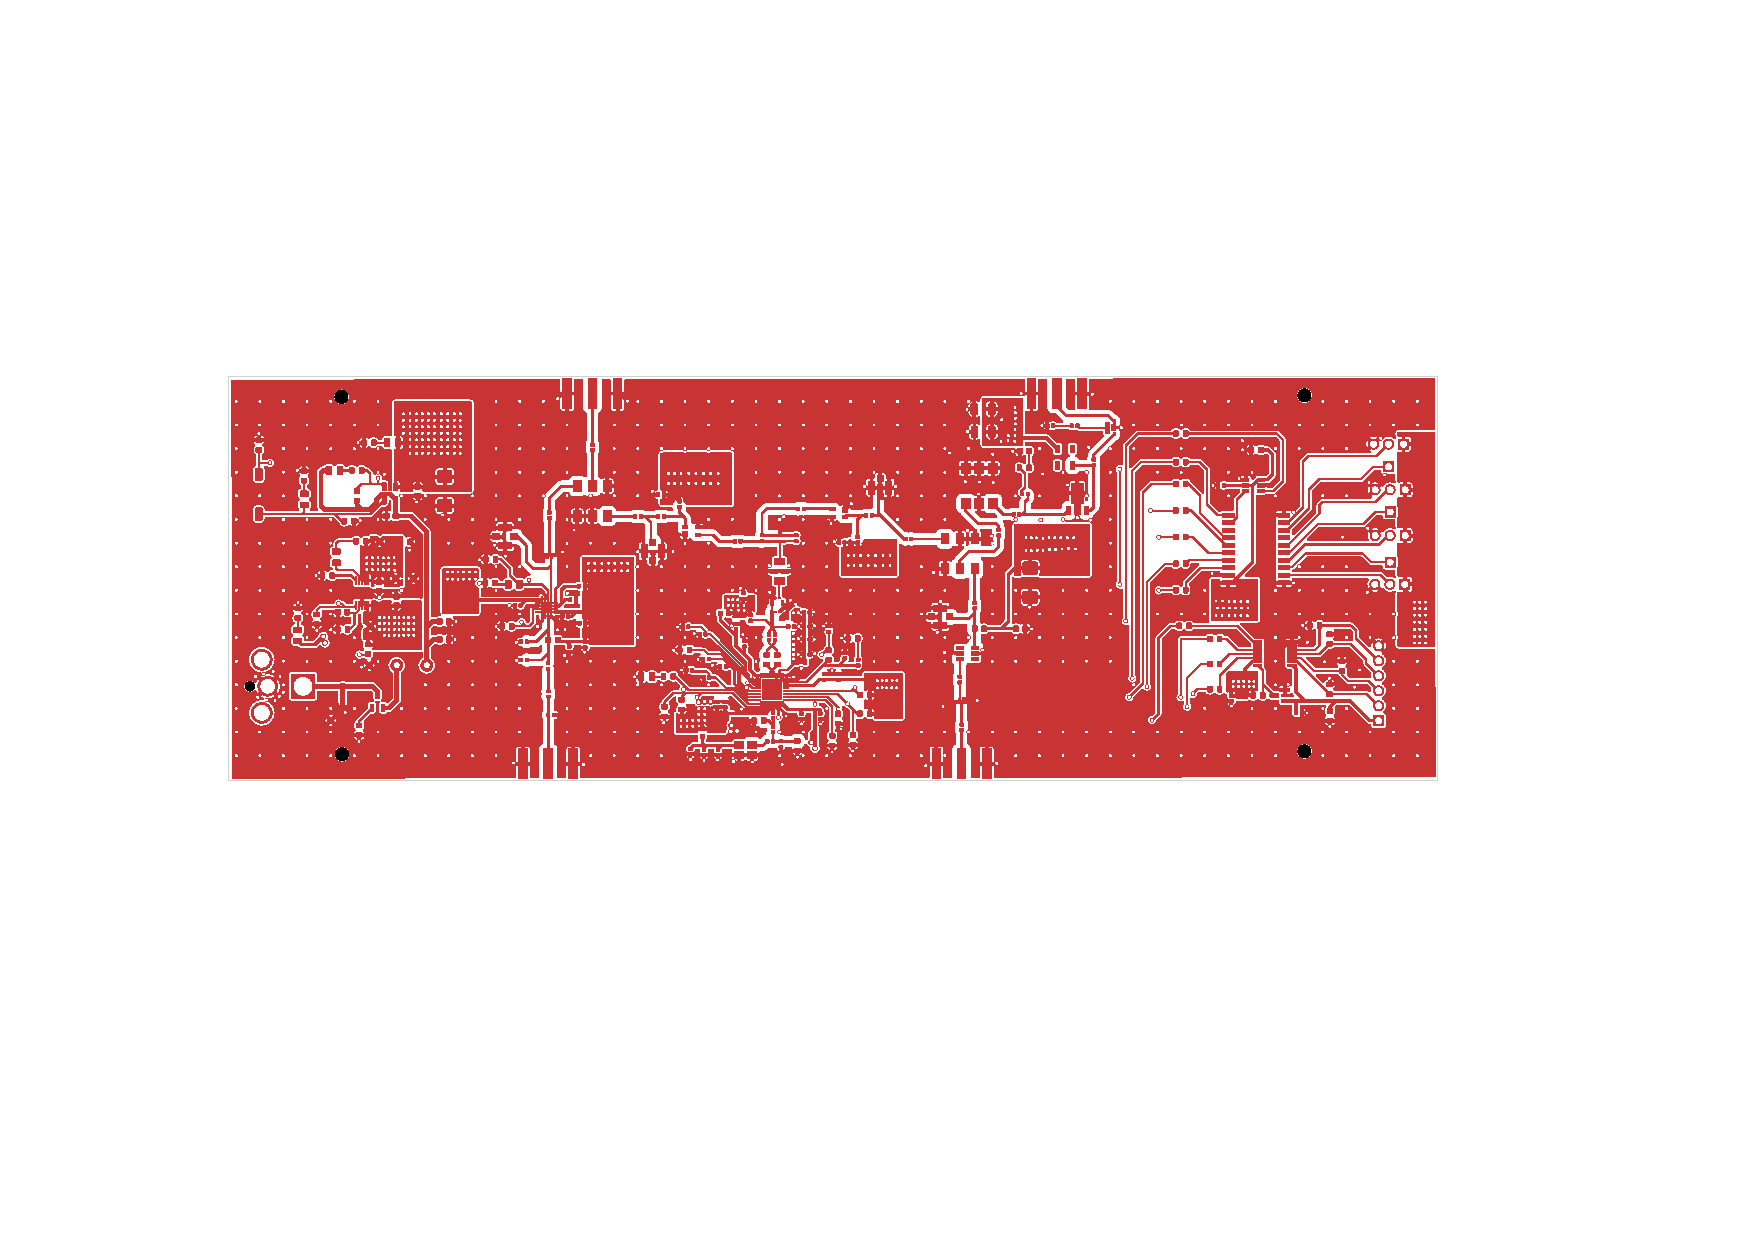
\includepdf[pages=-]{media/layout.pdf}

\end{document}